\documentclass[11pt,a4paper]{article}

\usepackage[margin=1in]{geometry}
\usepackage{amsmath,amssymb}
\usepackage{graphicx}
\usepackage{booktabs}
\usepackage{enumitem}
\usepackage{hyperref}
\usepackage{xcolor}
\usepackage{float}
\usepackage{microtype}

\setlength{\parindent}{0pt}
\setlength{\parskip}{0.5em}
\setlist[itemize]{nosep,leftmargin=*}
\setlist[enumerate]{nosep,leftmargin=*}

\title{\textbf{ID6002W : RL Course Project Report}\\[0.4em]
\large Industrial Inventory Control}
\author{Sohang Chopra \quad | \quad DA25M622}
\date{}

\begin{document}

\maketitle

\section{Problem and Assigned Configuration}

The industrial inventory control problem requires an agent to manage order quantities across three distinct products over discrete time steps to minimize total operational costs. The cost function penalizes holding excess stock, placing orders, discarding expired or overstocked units, and experiencing stockouts when demand exceeds available inventory. Stochastic customer demand and non-zero lead times create delayed arrivals, requiring policies to coordinate multi-echelon pipelines and capacity constraints.

\begin{itemize}
    \item \textbf{Project version:} \texttt{IITM-6002W-RL-Inventory-2026-v1}
    \item \textbf{Roll number:} \texttt{DA25M622}
    \item \textbf{Variant ID:} \texttt{V022}
    \item \textbf{Config fingerprint:} \texttt{7d77fc79debf206a}
    \item \textbf{Demand multiplier profile:} \texttt{[1.0, 1.1, 0.9]}
    \item \textbf{Initial inventory profile:} \texttt{[110, 100, 90]}
    \item \textbf{Lead-time delay profile:} \texttt{[0.1, 0.0, 0.05]}
\end{itemize}

\section{Techniques Attempted}

Five distinct reinforcement learning techniques were implemented and evaluated: Advantage Actor-Critic (A2C), Proximal Policy Optimization (PPO), Deep Q-Network (DQN), Double Deep Q-Network (Double DQN), and Monte Carlo Policy Gradient (REINFORCE with Baseline). 

\begin{table}[H]
\centering
\small
\begin{tabular}{p{0.20\textwidth}p{0.32\textwidth}p{0.44\textwidth}}
\toprule
\textbf{Technique} & \textbf{Observations Used} & \textbf{Key Design Choices} \\
\midrule
A2C & Dict observation: \texttt{inventory} (3), \texttt{arrival\_pipeline} (12), \texttt{demand\_history} (21), \texttt{day} (1), \texttt{capacity\_utilisation} (1) & Synchronous multi-step actor-critic using Stable-Baselines3 \texttt{MultiInputPolicy}, parallelized over 4 vectorized environments, shared feature extractor with separate policy and value heads. \\
\addlinespace[0.3em]
PPO & Same dictionary state representation (total 38 flattened scalar features) & Clipped surrogate objective with GAE; \texttt{MultiInputPolicy}; 4 parallel workers; minibatch updates with value function and entropy regularization terms. \\
\addlinespace[0.3em]
DQN & Flattened dictionary state vector mapped into a single observation array (38 features) & Discrete action space flattened from $\text{MultiDiscrete}([11, 11, 11])$ to $\text{Discrete}(1331)$ via action wrapper; experience replay buffer size 100,000; $\epsilon$-greedy exploration decay; target Q-network. \\
\addlinespace[0.3em]
Double DQN & Flattened state vector (38 features) & Same $\text{Discrete}(1331)$ action wrapper as DQN; decoupled action selection via online Q-network and action evaluation via target Q-network to eliminate Q-value overestimation bias. \\
\addlinespace[0.3em]
REINFORCE with Baseline & Dict converted to tensor: \texttt{inventory}, \texttt{arrival\_pipeline}, \texttt{demand\_history}, \texttt{day}, \texttt{capacity\_utilisation} & Custom PyTorch policy and value networks; 3-head categorical action output ($11 \times 3$ logits); parameterized baseline value network trained via MSE loss; normalized returns and gradient clipping. \\
\bottomrule
\end{tabular}
\caption{Summary of techniques attempted.}
\end{table}

\section{Training and Experimental Setup}

All models were evaluated under an identical protocol using a deterministic evaluation over 20 evaluation episodes, with the reward defined by the environment as $r_t = -\text{cost}_t / 100$. Random seed 2026 was fixed across environment instances, data generators, and network initializations. Hyperparameters for all five models were systematically tuned using Optuna's Tree-structured Parzen Estimator (TPE) sampler over 15 optimization trials each.

\begin{itemize}
    \item \textbf{Training steps/episodes:}
    \begin{itemize}
        \item A2C: 200,000 timesteps (final run) across 4 parallel environments.
        \item PPO: 200,000 timesteps (final run) across 4 parallel environments.
        \item DQN: 100,000 timesteps with 1,000 learning start steps.
        \item Double DQN: 80,000 timesteps with 500 learning start steps.
        \item REINFORCE with Baseline: 500 complete rollout episodes (1,000 max steps per episode).
    \end{itemize}
    \item \textbf{Discount factor and learning rates:}
    \begin{itemize}
        \item A2C: $\gamma = 0.995$, learning rate $= 1.04 \times 10^{-4}$, $\lambda_{\text{GAE}} = 0.95$.
        \item PPO: $\gamma = 0.99$, learning rate $= 2.50 \times 10^{-4}$, $\lambda_{\text{GAE}} = 0.90$, clip range $= 0.3$.
        \item DQN: $\gamma = 0.99$, learning rate $= 7.00 \times 10^{-4}$, batch size $= 64$.
        \item Double DQN: $\gamma = 0.99$, learning rate $= 5.00 \times 10^{-4}$, batch size $= 128$.
        \item REINFORCE: $\gamma = 0.99$, actor learning rate $= 3.00 \times 10^{-4}$, critic learning rate $= 5.00 \times 10^{-4}$.
    \end{itemize}
    \item \textbf{Exploration strategy:}
    \begin{itemize}
        \item DQN: $\epsilon$-greedy schedule decaying over an exploration fraction of 0.30 to a final $\epsilon = 0.05$.
        \item Double DQN: $\epsilon$-greedy schedule decaying over an exploration fraction of 0.25 to a final $\epsilon = 0.10$.
        \item A2C, PPO, and REINFORCE: Stochastic categorical sampling during training parameterized by action logits, assisted by entropy regularization (coefficients: $2.00 \times 10^{-4}$ for A2C, $0.01$ for PPO, and $0.01$ for REINFORCE).
    \end{itemize}
    \item \textbf{Reward shaping:} No artificial reward shaping was introduced; the environment default reward ($-\text{total\_cost} / 100$) was preserved to ensure uncorrupted policy convergence to the true cost objective. Advantage normalization was applied to policy gradient baselines.
    \item \textbf{Random seeds:} Seed 2026 was used as the universal master seed across training environments, policy network initialization, and evaluation seeds (\texttt{SEED + episode\_idx} for custom rollouts).
\end{itemize}

\section{Results}

Validation performance was measured across 20 deterministic evaluation episodes locally prior to leaderboard submission. Table 2 reports local evaluation performance alongside confirmed public leaderboard submission outcomes.

\begin{table}[H]
\centering
\small
\begin{tabular}{lrrrr}
\toprule
\textbf{Technique} & \textbf{Local Mean Cost} & \textbf{Public Leaderboard Cost} & \textbf{Submission ID} & \textbf{Network Architecture} \\
\midrule
PPO & 81,770.00 & 112,479.75 & 3418 & MLP [128, 128] \\
Double DQN & 104,805.00 & 134,677.50 & 3510 & MLP [128, 128] \\
DQN & 108,775.00 & 116,214.38 & 3551 & MLP [256, 256] \\
A2C & 153,264.25 & 154,022.75 & 3666 & MLP [256, 256] \\
REINFORCE w/ Baseline & 1,591,876.80 & 1,290,798.88 & 3621 & MLP [256, 128] \\
\bottomrule
\end{tabular}
\caption{Validation and public leaderboard performance across attempted techniques.}
\end{table}

\begin{figure}[H]
    \centering
    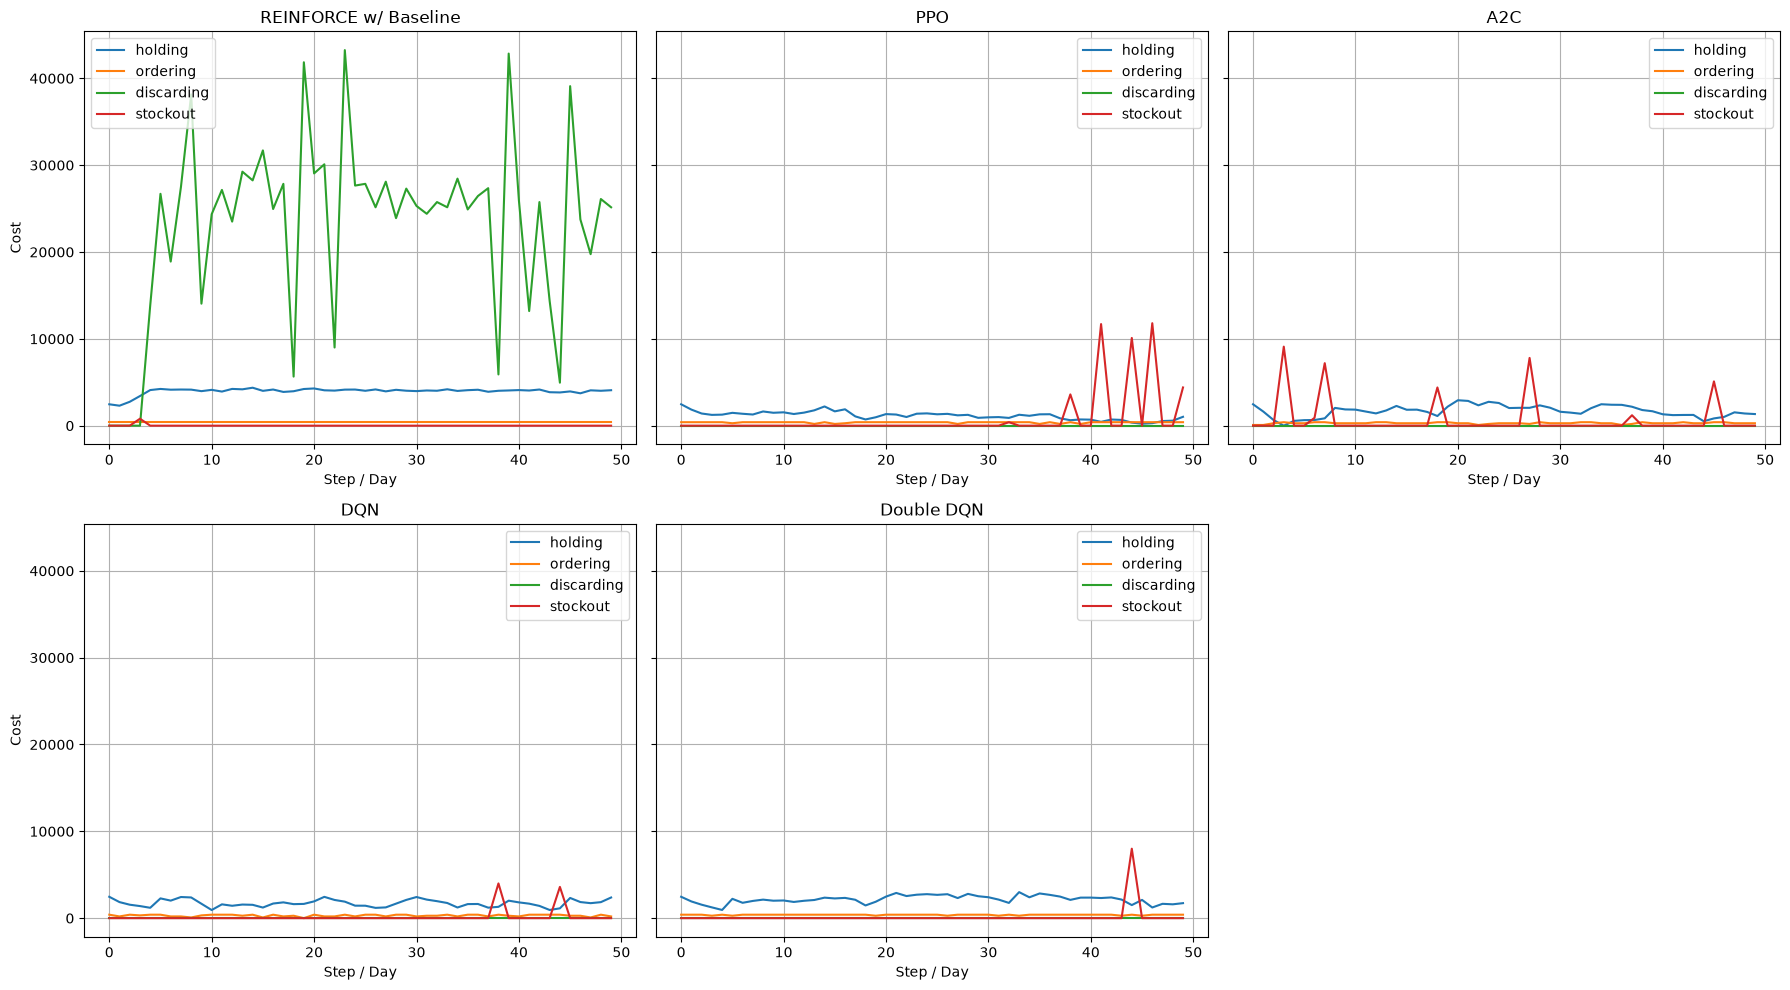
\includegraphics[width=0.85\textwidth]{all_models_cost_plots.png}
    \caption{Breakdown of cost components (holding, ordering, discarding, stockout) across time steps in an evaluation episode for all five models.}
\end{figure}

\section{Analysis and Observations}

\begin{itemize}
    \item \textbf{Comparative Performance:} PPO achieved the lowest overall cost (local mean of 81,770.00 and public score of 112,479.75). The clipped surrogate objective prevented destructive gradient updates, allowing steady policy refinement over multi-product action interactions.
    \item \textbf{Discrete Action Space Complexity:} Both DQN (local: 108,775.00) and Double DQN (local: 104,805.00) handled the $11^3 = 1331$ action space effectively, but the combinatorially large action space slowed convergence and increased sensitivity to target network update intervals ($1000$ to $2000$ steps). Double DQN reduced local mean cost compared to standard DQN by suppressing overestimation bias.
    \item \textbf{Value of Arrival Pipeline and State Features:} The observation vector consisted of 38 dimensions: current inventory (3), in-transit arrival pipeline (12), demand history (21), current day (1), and capacity utilization (1). Policies that successfully suppressed stockout and discard costs relied heavily on the arrival pipeline and demand history to anticipate deliveries and hedge against non-zero lead-time delays (up to 10\% delay probability for Product 0).
    \item \textbf{Failure Modes and Cost Profile Analysis:} As evidenced in Figure 1, the primary failure mode for weaker policies (such as REINFORCE with Baseline) was severe stockout spikes and high discard costs stemming from erratic ordering swings. A2C maintained relatively uniform ordering but incurred sustained holding costs due to over-buffering inventory. PPO established a tighter balance, maintaining low holding costs while rarely triggering stockouts or discards.
    \item \textbf{Sample Efficiency and High Variance:} REINFORCE with Baseline exhibited catastrophic variance and sample inefficiency, averaging costs above $1.2 \times 10^6$. Because Monte Carlo returns require full-trajectory rollouts without bootstrapping, policy updates were delayed and noisy compared to temporal difference and actor-critic methods.
\end{itemize}

\section{Key Learning}

\begin{enumerate}
    \item \textbf{Policy Gradient Stability with Clipping:} PPO's clipped objective and GAE advantage estimation significantly outperformed unclipped actor-critic (A2C) and Monte Carlo policy gradients (REINFORCE), proving essential for high-dimensional multi-product inventory balance.
    \item \textbf{Scalability Limits of Value-Based Methods on Joint Spaces:} Factoring a MultiDiscrete action space into a flat 1331-dimensional discrete space allows DQN/Double DQN to learn valid policies, but introduces severe sample complexity and high replay buffer requirements compared to multi-head actor policies.
    \item \textbf{Importance of Arrival Pipeline Tracking in Delayed MDPs:} In inventory environments with non-zero lead times, observing current on-hand stock alone is insufficient; pipeline tracking is critical to prevent redundant over-ordering and subsequent discard penalties.
    \item \textbf{Hyperparameter Sensitivity in RL Control:} Systematically tuning discount factor $\gamma$ close to 0.99--0.995 and applying entropy regularization was decisive in preventing premature convergence to sub-optimal policies like zero-ordering or excessive hoarding.
\end{enumerate}

\section*{References}

\begin{itemize}
    \item Schulman, J., Wolski, F., Dhariwal, P., Radford, A., \& Klimov, O. (2017). Proximal Policy Optimization Algorithms. \textit{arXiv preprint arXiv:1707.06347}.
    \item Mnih, V. et al. (2015). Human-level control through deep reinforcement learning. \textit{Nature}, 518(7540), 529--533.
    \item Van Hasselt, H., Guez, A., \& Silver, D. (2016). Deep Reinforcement Learning with Double Q-learning. In \textit{Proceedings of the AAAI Conference on Artificial Intelligence}, 30(1).
    \item Raffin, A., Hill, A., Gleave, A., Kanervisto, A., Ernestus, M., \& Dormann, N. (2021). Stable-Baselines3: Reliable Reinforcement Learning Implementations. \textit{Journal of Machine Learning Research}, 22(268), 1--8.
    \item Akiba, T., Sano, S., Yanase, T., Ohta, T., \& Koyama, M. (2019). Optuna: A Next-generation Hyperparameter Optimization Framework. In \textit{Proceedings of the ACM SIGKDD International Conference on Knowledge Discovery \& Data Mining}, 2623--2631.
\end{itemize}

\end{document}